

\begin{document}

\begin{frame}\frametitle{Outline}
\tableofcontents[pausesections,hidesubsections]
\end{frame}

\begin{frame}\frametitle{Resources}
\begin{itemize}
\item Unix for Beginners. Dirk Vermeir
\item \url{http://osl.iu.edu/~lums/swc/www/index.html}
\end{itemize}
\end{frame}

%\section{Questions \& Answers}

%\begin{frame}\frametitle{Q \& A}
%\begin{center}
%
\includegraphics[width=6cm,keepaspectratio]{question}
%\end{center}
%\end{frame}

%\section{Problem Solving}

%\begin{frame}\frametitle{Problem Solving}
%\begin{alertblock}{Problem 1}
%Functions for Mastermind
%\end{alertblock}
%\pause
%\begin{alertblock}{Problem 2}
%Sorting a list of numbers
%\end{alertblock}
%\end{frame}

\section{Shell Basics}

\subsection{The Shell}
\begin{frame}\frametitle{Why Command-line?}
\begin{itemize}
\item Most modern tools have a graphical user interface (GUI)
\begin{itemize}
    \item Because they're easier to use
\end{itemize}
\item But command-line user interfaces (CLUIs) still have their place
\begin{itemize}
    \item Easier (faster) to build new CLUI tools
\begin{itemize}
          \item Building a GUI takes time
          \item Building a good GUI takes a lot of time
\end{itemize}
    \item Higher action-to-keystroke ratio
\begin{itemize}
          \item Once you're over the (steeper) learning curve
\end{itemize}
    \item Easier to see and understand what the computer is doing on your behalf
\begin{itemize}
          \item Which is part of what this course is about
\end{itemize}
    \item Most important: it's easier to combine CLUI tools than GUI tools
\begin{itemize}
          \item Small tools, combined in many ways, can be very powerful
\end{itemize}
\end{itemize}
\end{itemize}
\end{frame}

\begin{frame}\frametitle{The Shell}
The most important command-line tool is the command shell (often just called “the shell”)
\begin{itemize}
    \item Manages a user's interactions with the operating system by:
\begin{itemize}
          \item Reading commands from the keyboard
          \item Figuring out what programs the user wants to run
          \item Running those programs
          \item Displaying their output on the screen
\end{itemize}
    \item Looks (and works) like an interactive terminal circa 1980
\end{itemize}
\end{frame}

\begin{frame}\frametitle{The Terminal}
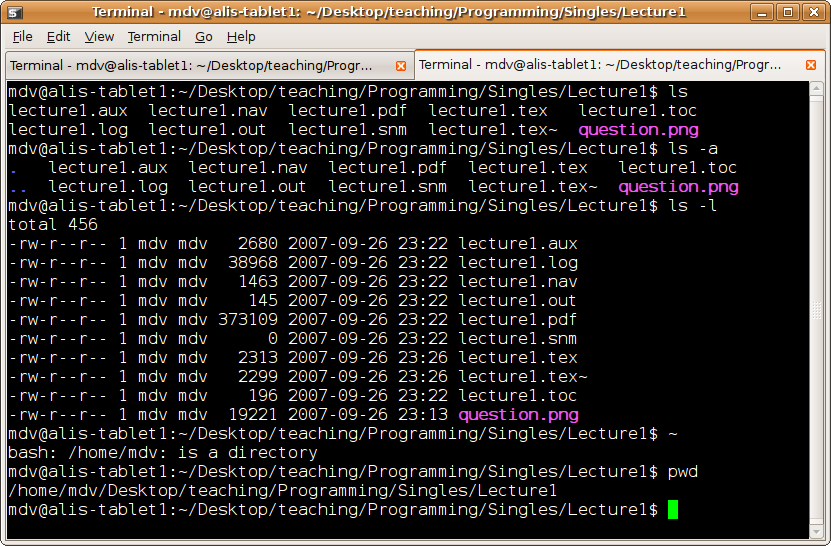
\includegraphics[height=7.5cm,keepaspectratio]{terminal}
\end{frame}

\begin{frame}\frametitle{The Shell vs. the Operation System}

\begin{itemize}
\item The shell is just one program among many
\begin{itemize}
    \item Many different ones have been written
    \item \keytext{sh} was the first for Unix
	\begin{itemize}
          \item Most others extend its capabilities in various ways
          \item Which means that it's the lowest common denominator you can always rely on
	\end{itemize}
    \item We will use \keytext{bash} (the Bourne again shell)
\begin{itemize}
          \item Available just about everywhere
          \item Even on Windows (thanks to Cygwin)
\end{itemize}
\end{itemize}
\end{itemize}
\end{frame}
\begin{frame}\frametitle{The Shell vs. the Operation System}
\begin{itemize}
\item In contrast, the operating system is not just another program
\begin{itemize}
    \item Automatically loaded when the computer boots up
    \item The only program that can talk directly to the computer's hardware
\begin{itemize}
          \item I.e., read characters from the keyboard, or send drawing commands to the screen
\end{itemize}
    \item Manages files and directories on the disk
    \item Keeps track of who you are, and what you're allowed to do
    \item You can run many instances of the shell on a computer at once, but it can only run one operating system at a time
\end{itemize}
\end{itemize}
\end{frame}

\subsection{The File System}

\begin{frame}\frametitle{The File System}
\begin{itemize}
\item The file system is the set of files and directories the computer can access
\begin{quote}
     “Everything that stays put when you turn the computer off and restart it”
\end{quote}
\item Data is stored in files
\begin{itemize}
    \item By convention, files have two part names, like notes.txt or home.html
    \item Most operating systems allow you to associate a filename extension with an application
\begin{itemize}
          \item E.g., .txt is associated with an editor, and .html with a web browser
\end{itemize}
    \item But this is all just convention: you can call files (almost) anything you want
\end{itemize}
\item Files are stored in directories (often called folders)
\begin{itemize}
    \item Directories can contain other directories, too
    \item Results in the familiar directory tree
\end{itemize}
\end{itemize}
\end{frame}

\begin{frame}\frametitle{Directory Tree}
\begin{tikzpicture}[edge from parent fork down, scale=0.8]
\tikzstyle{every node}=[shade, ball color=\lightrow]
\tikzstyle{edge from parent}=[color=\darkrow,-o,thick,draw]
\node {/}
    child {node {usr}             
          child {node {bin}}
          child {node {lib}}
          child {node {man}}
          child {node {sbin}}
          child {node {slocal}
             child {node {bin}
                 child {node {bash}}
             }
             child {node {src}}
             child {node {lib}}
          }
    } 
    child {node {dev}}
    child {node {etc}}
    child {node {...}}
    child {node {...}}
    child {node {export}
        child {node {home}
           child {node {marinadv}
	       child {node {.bashrc}}
	       child {node {...}}
               child {node {.src}
                  child {node {uintro.pdf}}
               }		
           } 
        }
    }
    child {node {...}}
;
\end{tikzpicture}

\end{frame}

\begin{frame}[fragile]\frametitle{Drives}
\begin{itemize}
\item On Unix, the file system has a unique \keytext{root directory} called \lstinline!/!
\begin{itemize}
    \item Every other directory is a child of it, or a child of a child, etc.
\end{itemize}
\item On Windows, every \keytext{drive} has its own root directory
\begin{itemize}
    \item So \lstinline!C:\home\mdv\notes.txt! is different from \lstinline!J:\home\mdv\notes.txt!
    \item When you're using Cygwin, you can also write \lstinline!C:home\mdv! 
 as \lstinline!c:/home/mdv!
    \item Or as \lstinline!/cygdrive/c/home/mdv!
\begin{itemize}
          \item Some Unix programs give ":" a special meaning, so Cygwin needed a way to write paths without it…
\end{itemize}
\end{itemize}
\end{itemize}
\end{frame}

\begin{frame}[fragile]\frametitle{Paths}
A \keytext{path} is a description of how to find something in a file system
\begin{itemize}
    \item An \keytext{absolute path} describes a location from the root directory down
\begin{itemize}
          \item Equivalent to a street address
          \item Always starts with "/"
          \item E.g., \lstinline{/home/mdv} is my home directory, and \lstinline{/courses/swc/lec/shell.swc} is this file
\end{itemize}
    \item A \keytext{relative path} describes how to find something from some other location
\begin{itemize}
          \item Equivalent to saying, “Four blocks north, and seven east”
          \item E.g., from \lstinline!/courses/swc!, the relative path to this file 
	is \lstinline!lec/shell.swc!
\end{itemize}
\end{itemize}
\end{frame}

\begin{frame}[fragile]\frametitle{Special Paths}
\begin{itemize}
\item Every program (including the shell) has a current working directory
\begin{itemize}
    \item “Where am I?”
    \item Relative paths are deciphered relative to this location
    \item It can change while a program is running
\end{itemize}
\item Finally, two special names:
\begin{itemize}
    \item "." means “the current directory”
    \item ".." means “the directory immediately above this one
\begin{itemize}
          \item Also called the parent directory
          \item In \lstinline!/courses/swc/data!, .. is \lstinline!/courses/swc!
          \item In \lstinline!/courses/swc/data/elements!, .. is \lstinline!/courses/swc/data!
\end{itemize}
\end{itemize}
\end{itemize}
\end{frame}

\begin{frame}\frametitle{File Systems}
Most unix systems have several types of file systems
\begin{itemize}
\item Disk-based: UFS : to store all the files users create
\item Netword-based: NFS: to connect to (mount) drives outside the machine
\item tmpfs file system: supports simulating a file system in main memory, possibly backed up by swap storage. This is ideal for temporary files for which
fast access is important.
\item swap: 
file system is used to provide backup storage for processes that must
temporarily be “swapped out”
\item  proc file space: provides a “file view” on the attributes of processes
\end{itemize}
\end{frame}

\subsection{Some Linux Commands}

\begin{frame}[fragile]\frametitle{pwd and ls}
\begin{itemize}
\item \keytext{\lstinline!pwd!} shows you the current directory
\end{itemize}
\codelist
\begin{lstlisting}
pwd
\end{lstlisting}
\reslist
\begin{lstlisting}
/home/mdv/Desktop/teaching/Programming/Singles/Lecture1
\end{lstlisting}
\begin{itemize}
\item \keytext{\lstinline!ls!} shows you what's in the current directory
\end{itemize}
\codelist
\begin{lstlisting}
ls
\end{lstlisting}
\reslist
\begin{lstlisting}
lecture1.aux  lecture1.out  lecture1.tex   lecture1.vrb
lecture1.log  lecture1.pdf  lecture1.tex~  question.png
lecture1.nav  lecture1.snm  lecture1.toc   terminal.png
\end{lstlisting}
\end{frame}

\begin{frame}[fragile]\frametitle{More on ls}
What actually happens when I type ls is:
\begin{itemize}
    \item The operating system reads characters from the keyboard
    \item Passes them to the shell (because it's the currently active window on my desktop)
    \item The shell breaks the line of text it receives into words
    \item Looks for a program with the same name as the first word (i.e., the command to run)
\begin{itemize}
          \item Describe in a moment how the shell knows where to look
\end{itemize}
    \item Runs that program
    \item Reads the program's output and sends it back to the operating system for display
\end{itemize}
\end{frame}

\begin{frame}[fragile]\frametitle{Flags}
\begin{itemize}
\item \keytext{Flags are command-line option you can pass to commands}
\item Can tell ls to produce more informative output by giving it some flags
\item By convention, flags start with "-", as in "-c" or "-l"
\item For example: show directories with trailing slash
\end{itemize}
\codelist
\begin{lstlisting}
ls -F
\end{lstlisting}
\reslist
\codesmall
\begin{lstlisting}
bluej.png     code.sty~       copyright.tex~  rights.png     uintro.pdf
cm10192.tex   computer.jpg    Doubles/        Singles/
cm10192.tex~  computer.png    projects.zip    Stylefiles/
code.sty      copyright.tex*  python.png      template.tex~
\end{lstlisting}
\begin{itemize}
\item -a: gives you all files starting with ".", which are normally hidden
\item -l: provides long listing format. provides permissions,size,latest access
\end{itemize}
\end{frame}

\begin{frame}[fragile]\frametitle{Finding your way}
\begin{itemize}
\item man pages: provide an overview of the functionality of a command.
\begin{itemize}
\item \lstinline!man ls!
\end{itemize}
\end{itemize}
\begin{itemize}
\item apropos: provides all commands related to a certain topic
\begin{itemize}
\item \lstinline!appropos(permissions)!
\end{itemize}
\end{itemize}
\begin{itemize}
\item \lstinline!--help!: provides support for a specific command
\begin{itemize}
\item \lstinline!ls --help!
\end{itemize}
\end{itemize}
\end{frame}

\begin{frame}[fragile]\frametitle{Manipulating Files and Directories}
Lets work by example:
\begin{itemize}
\item let us create a temporary directory and play around in there
\end{itemize}
\codelist
\begin{lstlisting}
      mkdir temp
\end{lstlisting}
\begin{itemize}
    \item Note: no output
    \item The -v (“verbose”) flag tells mkdir to print a confirmation message
\item Now go into that directory
\end{itemize}
\begin{lstlisting}
      cd temp
\end{lstlisting}
\begin{itemize}
\item Changes the shell's notion of our current working directory
\end{itemize}
\begin{lstlisting}
      pwd
\end{lstlisting}
\reslist
\begin{lstlisting}
      /home/mdv/programming1/temp
\end{lstlisting}
\end{frame}

\begin{frame}[fragile]\frametitle{Manipulating Files and Directories II}
\begin{itemize}
\item No files there yet:
\end{itemize}
\codelist
\begin{lstlisting}
      ls -a
\end{lstlisting}
\reslist
\begin{lstlisting}
      . ..
\end{lstlisting}
\begin{itemize}
\item Use the editor of your choice (emacs,vim) to create a file called earth.txt with the following contents:
\codesmall
\fbox{\footnotesize{\texttt{\begin{tabular}{l}
Name: Earth\\
Period: 365.26 days\\
Inclination: 0.00\\
Eccentricity: 0.02\\
Object: Planet\\
\end{tabular}}}}
\end{itemize}
\end{frame}

\begin{frame}[fragile]\frametitle{Manipulating Files and Directories III}
\begin{itemize}
\item Easiest way to create a similar file venus.txt is to copy the one we have
\end{itemize}
\codelist
\begin{lstlisting}
      cp earth.txt venus.txt
\end{lstlisting}
\codelist
\begin{lstlisting}
      ls -t
\end{lstlisting}      
\reslist
\begin{lstlisting}
      venus.txt   earth.txt
\end{lstlisting}
\begin{itemize}      
    \item Note: the -t option tells ls to list newest first
    \item Check the contents of the file using \lstinline!cat! (short for “concatenate”)
    \item Just prints the contents of a file to the screen
    \item You can also use \lstinline!more! or \lstinline!less!
\end{itemize}	
\end{frame}

\begin{frame}[fragile]\frametitle{Manipulating Files and Directories IV}
\begin{itemize}
\item Edit the file so that looks like:
\fbox{\footnotesize{\texttt{\begin{tabular}{l}
Name: Venus\\
Period: 224.70 days\\
Inclination: 3.39\\
Eccentricity: 0.01\\
Object: Planet
\end{tabular}}}}
\codenormal
\item Compare the sizes of the two files using \lstinline!wc! (for “word count”) and 
Compare the two files using \lstinline!diff!
\end{itemize}
\codesmall
\reslist
\begin{multicols}{2}
\begin{lstlisting}[linewidth=5cm]
wc earth.txt venus.txt

  4   9  69 earth.txt
  4   9  69 venus.txt
  8  18 138 total
\end{lstlisting}
\mbox{}\\
\mbox{}\\
\mbox{}\\
\mbox{}\\
\begin{lstlisting}[linewidth=5cm]
diff earth.txt venus.txt

1,4c1,4
< Name: Earth
< Period: 365.26 days
< Inclination: 0.00
< Eccentricity: 0.02
---
> Name: Venus
> Period: 224.70 days
> Inclination: 3.39
> Eccentricity: 0.01
\end{lstlisting}
\end{multicols}
\end{frame}

\begin{frame}[fragile]\frametitle{Manipulating Files and Directories V}
\begin{itemize}
\item Linux does not care about filename extensions.
\item \lstinline!cp earth.txt earth.pdf! is valid although not a very sensible thing to do
\item we can rename it using \lstinline!mv earth.pdf earth2.txt!
\item Removing a file can be done using \lstinline!rm!, like for example \lstinline!rm earth2.txt!
\item A empty directory can be removed with \lstinline!rmdir! or \lstinline!rm -r! which recursively removed all files.
\end{itemize}
\end{frame}

\begin{frame}[fragile]\frametitle{Wildcards}
\begin{itemize}
\item Some characters (\keytext{wildcards}) mean special things to the shell
\begin{itemize}
    \item * matches zero or more characters
\begin{itemize}
          \item So ls *.f77 lists all the Fortran-77 files in a directory
\end{itemize}
\codesmall
\codelist
\begin{lstlisting}[linewidth=6cm]
      wc *.txt

        4   9  69 earth.txt
        4   9  69 venus.txt
        8  18 138 total
\end{lstlisting}
\codenormal
    \item ? matches any single character
\begin{itemize}
          \item So \lstinline!ls ??.txt! lists all the text files with two-letter prefixes
          \item And \lstinline!ls ??.*! lists all the files with two-letter prefixes, and any extension
\end{itemize}
    \item ~ on its own means “the users home directory”
    \item ~harry means “Harry's home directory”
\end{itemize}
\item Note: the shell expands wildcards before running commands
\item Note: Be careful using \lstinline!rm! in conjunction with *
\end{itemize}
\end{frame}

\begin{frame}[fragile]\frametitle{Users}
\begin{itemize}
\item Users have a \keytext{user name} and a \keytext{password}
\item a user also has a \keytext{home directory}, and a \keytext{shell program}.
\item Internally, the system uses so-called \keytext{UID} numbers to identify users.
\item All this information is stored in the file \keytext{/etc/passwd}
\item This also stores the user “primary” group id (GID) identifying a group to which the user belongs.
\item A \keytext{group} is an arbitrary set of users
\item A user can belong to several groups
\item \lstinline!whoami!,\lstinline!users!,\lstinline!groups! provide you with information regarding users and groups
\item There is one special user with UID 0, called \keytext{root}
\item This user is often called the
“super user” because he can access all resources on the system, independently of
any specific permissions
\end{itemize}
\end{frame}

\begin{frame}[fragile]\frametitle{Ownership}
\begin{itemize}
\item Each file has a user as \keytext{owner} and a group as \keytext{group owner}.
\item Using \lstinline{chmod} the owner can change  permissions that determine the type of access (read,
write or execute) ...
\item allowed to three categories of users: the owner herself, the users
belonging to the group owner group, and all other users.
\item Note that ''execute'' permission on a directory is interpreted as ''permission to traverse''
\end{itemize}
\codesmall
\reslist
\begin{lstlisting}
ls -l

-rw-r--r-- 1 mdv mdv     84 2007-09-27 23:08 earth.pdf

chmod g+w earth.txt
ls -l

-rw-rw-r-- 1 mdv mdv     84 2007-09-27 22:38 earth.txt
\end{lstlisting}
\end{frame}

\end{document}
